%
%このファイルは日本バーチャルリアリティ学会論文集用スタイルファイル
%jvrst2e.sty(ver.2.0) を利用したサンプルファイルです。

\documentclass[a4paper,twoside]{jarticle}
   \usepackage{style/tvrsj2e}
   % \usepackage[dvips]{graphicx}
   \usepackage[dvipdfmx]{graphicx}
   \usepackage{style/listings,style/jlisting} %日本語のコメントアウトをする場合jlistingが必要
   \usepackage{here}

%和文タイトル 論文のヘッダ部分にも出力されます。 
\jtitle{
    計算物理演習レポート1 モンテカルロ法}

%著者日本名
\jauthor{}

% ヘッダー
\header{計算物理演習レポート1 モンテカルロ法}

%論文の種別に合わせる
\TYPE{レポート}
%\TYPE{基礎論文}
%\TYPE{応用論文}
%\TYPE{コンテンツ論文}
%\TYPE{総説論文}
%\TYPE{ショートペーパー}

%ここからソースコードの表示に関する設定
\lstset{
  basicstyle={\ttfamily},
  identifierstyle={\small},
  commentstyle={\smallitshape},
  keywordstyle={\small\bfseries},
  ndkeywordstyle={\small},
  stringstyle={\small\ttfamily},
  frame={tb},
  breaklines=true,
  columns=[l]{fullflexible},
  numbers=left,
  xrightmargin=0zw,
  xleftmargin=3zw,
  numberstyle={\scriptsize},
  stepnumber=1,
  numbersep=1zw,
  lineskip=-0.5ex
}
%ここまでソースコードの表示に関する設定

\begin{document}

%maketitle は abstract と keyword の後に入れてください。

\maketitle

\section{概要}
モンテカルロ法とは数値計算を乱数を用いて行う手法の総称\cite{wiki-monte-carlo}である。今回はこのモンテカルロ法を用いてn次元球の体積を導出する。

なお、各値の計算には C++ 14、プロットには Python 3 の matplotlib を用いた。また、乱数の計算には MT 法を用いた。

\section{2次元においてのプロット}\label{s-2d}

\subsection{内容}
まずは2次元球、つまり円の場合において、$x: [0, 1)$, $y: [0, 1)$ にランダム点を打ったものをプロットした。

\subsection{ソースコード}

sphere2d.cpp
% \begin{lstlisting}[caption=hoge,label=fuga]
% \begin{figure}[t]
\begin{lstlisting}[]
#include <iostream>
//#include <cstdlib>
#include <cmath>
#include <random>
#include <fstream>
#include <string>
#include "util.h"

using namespace std;

int main() {
    int n = int(pow(10, 5)), d = 2, count = 0, interval = pow(10, 4);
    double r2s[n];
    string s;
    for (int i = 0; i < n; i++) {
        double r2 = 0.0;
        for (int j = 0; j < d; j++) {
            double x_j = get_random_0_to_1();
            r2 += pow(x_j, 2);
            if (j == 0) {
                s += to_string(x_j) + ",";
            } else {
                s += to_string(x_j) + "\n";
            }
        }
        if (r2 <= 1) count++;
        if (i % interval == interval - 1 or i == n - 1) {
            r2s[i] = r2;
            double v = double(count) / double(i + 1) * pow(2, d);
            double p = double(count) / double(i + 1);
            double q = 1.0 - p;
            double error = 1.96 * pow(2, d) * sqrt(p * q / double(i + 1));
            cout << "i + 1 = " << i + 1 << " v = " << v << " ± " << error << "\n";
        }
    }
    write_to_file(s, "../out/x_y_plot_2d.csv");
}
\end{lstlisting}
% \end{figure}

util.cpp
\begin{lstlisting}
//#include <random>
#include "Sample.h"

using namespace std;
\end{lstlisting}

util.h
\begin{lstlisting}
#pragma once

#include <fstream>
#include <random>

using namespace std;

inline double get_random_0_to_1() {
  // 乱数生成器
  static mt19937_64 mt64(0);

  // [0.0, 1.0) の一様分布実数生成器
  uniform_real_distribution<double> get_rand_uni_real(0.0, 1.0);
  // 乱数を生成
  return get_rand_uni_real(mt64);
}

inline int write_to_file(const string& s, const string& fpath) {
  ofstream f;
  f.open(fpath);
  f << s;
  f.close();
  return 0;
}
\end{lstlisting}

plot2d.py
\begin{lstlisting}
# -*- coding: utf-8 -*-

import matplotlib.pyplot as plt
import numpy as np
import csv

def main():
  data = []
  with open("../../cpp/out/x_y_plot_2d.csv") as f:
      rows = csv.reader(f, quoting=csv.QUOTE_NONNUMERIC)
      for row in rows:
          data.append(row)

  # print(data)
  x = [row[0] for row in data]
  y = [row[1] for row in data]
  plt.plot(x, y, 'b+', markersize=0.1)

  theta = np.linspace(0, np.pi / 2, 100)
  r = np.sqrt(1.0)
  circle_x = r * np.cos(theta)
  circle_y = r * np.sin(theta)
  plt.plot(circle_x, circle_y, 'black')

  plt.axes().set_aspect('equal', 'datalim')
  plt.grid(True, which="both", axis='both', ls="--", color="g")
  plt.xlabel('x')
  plt.ylabel('y')
  plt.savefig('out/plot2d.pdf')
  plt.savefig('out/plot2d.png')
  plt.show()


if __name__ == "__main__":
  main()

\end{lstlisting}

\subsection{結果}
C++ コンソール

\begin{lstlisting}[numbers=none]
i + 1 = 10000 v = 3.1444 ± 0.0321485
i + 1 = 20000 v = 3.142 ± 0.0227556
i + 1 = 30000 v = 3.14307 ± 0.0185714
i + 1 = 40000 v = 3.1426 ± 0.0160865
i + 1 = 50000 v = 3.13664 ± 0.0144245
i + 1 = 60000 v = 3.13553 ± 0.0131738
i + 1 = 70000 v = 3.13543 ± 0.0121971
i + 1 = 80000 v = 3.13605 ± 0.0114064
i + 1 = 90000 v = 3.13809 ± 0.0107448
i + 1 = 100000 v = 3.13872 ± 0.0101907

Process finished with exit code 0
\end{lstlisting}

\begin{figure}[ht]
\begin{center}
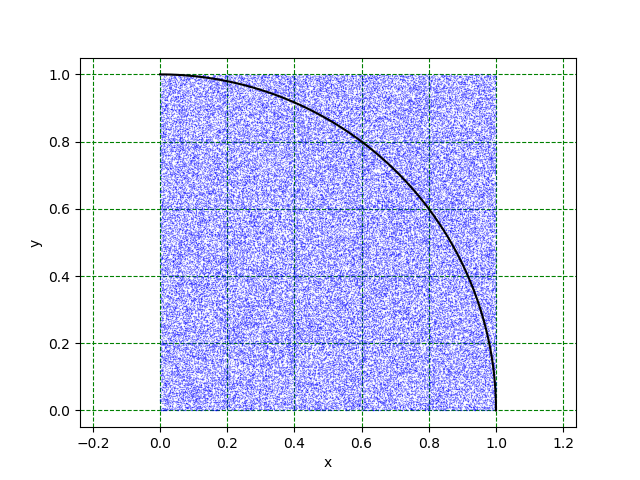
\includegraphics[width=8cm]{../python/report1_monte_carlo/out/plot2d.png}
\end{center}
\caption{2次元においてのランダム点プロット}
\label{fig:2d}
\end{figure}

\subsection{考察}
プロットされた点は偏りがなく、均等でなく見えるため、ランダムに点が打たれているできているといえる。乱数の評価という点において、MT 法によって生成された(疑似)乱数がモンテカルロ法を使うにあたって妥当であることが目視的に確認できる。

\section{分散の収束}\label{s-variance}
\subsection{内容}
分散が次第に小さくなっていき、超球の体積が理論値へ収束してくことを視覚的に確認する。次元は2次元から20次元までとし、試行回数は1億回、x軸のみ対数グラフとしてプロットした。

求める超球の体積は次元を$d$とすると、
\begin{equation}
  V_n(R)=2^d\frac{\textrm{(球の中に入った点の個数)}}{\textrm{(試行回数)}}
\end{equation}
と表せる。

求めた超球の体積の誤差は、$p=$(球の中に入った点の個数)/試行回数、$n=$試行回数として、
\begin{equation}
1.96\sigma=2^d\sqrt{\frac{p\left(1-p\right)}{n}}
\end{equation}
と95\%信頼区間で求めた。

理論値は超球の体積の公式\cite{wiki-volume-n-ball}
\begin{equation}
V_n(R)=\frac{\pi^{n/2}}{\Gamma\left(\frac{n}{2}+1\right)}R^n
\end{equation}
を用いた

\subsection{ソースコード}
sphere\_multi.cpp
\begin{lstlisting}
//#include <iostream>
#include <cmath>
#include <tuple>
#include "Sample.h"

using namespace std;

inline tuple<double, double, double, double> calc(int d, int i, int count) {
  double v = double(count) / double(i + 1) * pow(2, d);
  double p = double(count) / double(i + 1);
  double q = 1.0 - p;
  double error = 1.96 * pow(2, d) * sqrt(p * q / double(i + 1));
  return forward_as_tuple(v, p, q, error);
}

inline int main_inline() {
  const int n_pow = 8, n = int(pow(10, n_pow)), num_plot = 100, interval = n / num_plot;
  const int d_max = 20;
  string v_s;

  for (int d = 2; d <= d_max; d++) {
      double v_theory = pow(M_PI, double(d) / 2.0) / tgamma(double(d) / 2.0 + 1.0);

      int i_log = 0, count = 0;
      double r2s[n];
      string s;
      for (int i = 0; i < n; i++) {
          Sample sample(d);
          if (sample.run()) count++;

          double log10_i = log10(i + 1);
          if (log10_i >= double(n_pow) / double(num_plot) * double(i_log) or i == n - 1) {
              r2s[i] = sample.r2;
              double v, p, q, error;
              tie(v, p, q, error) = calc(d, i, count);
              printf("d = %d, i + 1 = %d, v = %f ± %f\n", d, i + 1, v, error);
              s += to_string(i + 1) + "," + to_string(v) + "," + to_string(error) + "," +
                      to_string(v_theory) + "\n";
              i_log++;
          }
          if (i + 1 == int(pow(10, 8))) {
              double v, error;
              tie(v, ignore, ignore, error) = calc(d, i, count);
              v_s += to_string(d) + "," + to_string(v) + "," + to_string(error) + "\n";
          }
      }
      string fpath = "../out/r2_plot_" + to_string(d) + "d.csv";
      write_to_file(s, fpath);
  }

  string v_s_path = "../out/v_s_plot.csv";
  write_to_file(v_s, v_s_path);

  return 0;
}

int main() {
  clock_t start = clock();

  main_inline();

  clock_t end = clock();
  const double time = double(end - start) / CLOCKS_PER_SEC;
  printf("Process finished. (%2.1f s)\n", time);

  return 0;
}
\end{lstlisting}

Sample.cpp
\begin{lstlisting}
//#include <cmath>
#include "Sample.h"
//#include "util.h"

Sample::Sample(int d) {
  this->d = d;
  this->r2 = 0.0;
}

Sample::~Sample() = default;
\end{lstlisting}

Sample.h
\begin{lstlisting}
#include <cmath>
#include "util.h"

class Sample {
private:
  int d;

public:
  explicit Sample(int d);
  ~Sample();

  bool run();

  double r2;
};

inline bool Sample::run() {
  for (int j = 0; j < d; j++) {
      double x_j = get_random_0_to_1();
      r2 += pow(x_j, 2);
      if (r2 > 1) return false;
  }
  return true;
}
\end{lstlisting}

util.cpp、util.h は\ref{s-2d}と同一である。

plotmulti.py
\begin{lstlisting}
# -*- coding: utf-8 -*-

import matplotlib.pyplot as plt
import numpy as np
import csv

from matplotlib import ticker


def loop(d: int):
  data = []
  with open("../../cpp/out/r2_plot_{}d.csv".format(d)) as f:
      rows = csv.reader(f, quoting=csv.QUOTE_NONNUMERIC)
      for row in rows:
          data.append(row)

  # print(data)
  n = [row[0] for row in data]
  v = [row[1] for row in data]
  error = [row[2] for row in data]
  v_theory = [row[3] for row in data]
  v_plus_error = [e + error[i] for i, e in enumerate(v)]
  v_minus_error = [e - error[i] for i, e in enumerate(v)]

  plt.plot(n, v, 'b', linestyle='solid')
  plt.plot(n, v_theory, 'r', linestyle='solid')
  # plt.plot(n, v_plus_error, 'b', linestyle='solid')
  # plt.plot(n, v_minus_error, 'b', linestyle='solid')
  plt.fill_between(n, v_plus_error, v, facecolor='lightblue')
  plt.fill_between(n, v, v_minus_error, facecolor='lightblue')

  # plt.axes().set_ylim(ymin=-max(v)*0.1, ymax=max(v_plus_error)*1.1)
  plt.axes().set_ylim(ymin=-0.1*v_theory[0], ymax=2.1*v_theory[0])
  plt.xscale('log')
  # plt.yscale('log')
  plt.grid(True, which="both", axis='both', ls="--", color="g")
  plt.xlabel('n')
  # plt.ylabel('v')
  plt.title('d = {}'.format(d))
  plt.savefig('out/r2plot{}d.eps'.format(d))
  plt.savefig('out/r2plot{}d.png'.format(d))
  plt.show()


def main():
  for d in range(2, 21):
      loop(d)


if __name__ == "__main__":
  main()
\end{lstlisting}

\subsection{結果}
C++ コンソール:(長文より冒頭のみ)
\begin{lstlisting}[numbers=none]
d = 2, i + 1 = 1, v = 0.000000 ± 0.000000
d = 2, i + 1 = 2, v = 2.000000 ± 2.771859
d = 2, i + 1 = 3, v = 2.666667 ± 2.133778
d = 2, i + 1 = 4, v = 3.000000 ± 1.697410
d = 2, i + 1 = 5, v = 2.400000 ± 1.717658
d = 2, i + 1 = 6, v = 2.666667 ± 1.508809
d = 2, i + 1 = 7, v = 2.857143 ± 1.338656
d = 2, i + 1 = 8, v = 3.000000 ± 1.200250
d = 2, i + 1 = 9, v = 2.666667 ± 1.231937
d = 2, i + 1 = 10, v = 2.800000 ± 1.136124
\end{lstlisting}

\begin{figure}[H]
\begin{center}
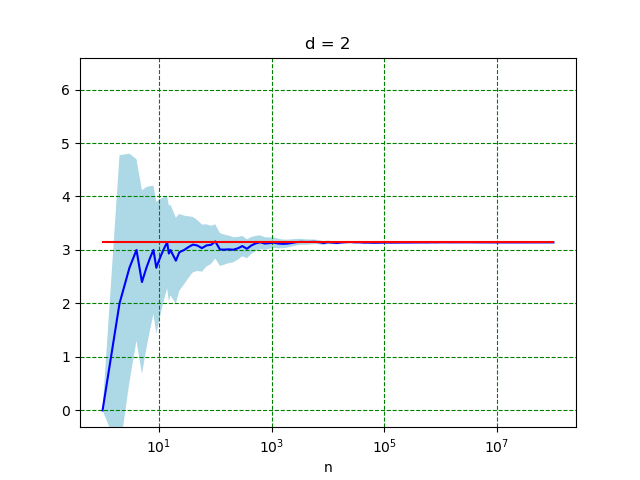
\includegraphics[width=8cm]{../python/report1_monte_carlo/out/r2plot2d.png}
\end{center}
\caption{2次元球の体積が理論値へと収束していく様子}
\end{figure}

\begin{figure}[H]
\begin{center}
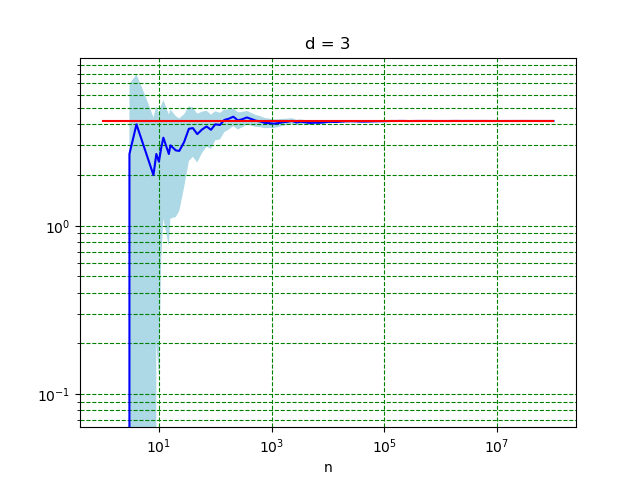
\includegraphics[width=8cm]{../python/report1_monte_carlo/out/r2plot3d.png}
\end{center}
\caption{3次元球の体積が理論値へと収束していく様子}
\end{figure}

\begin{figure}[H]
\begin{center}
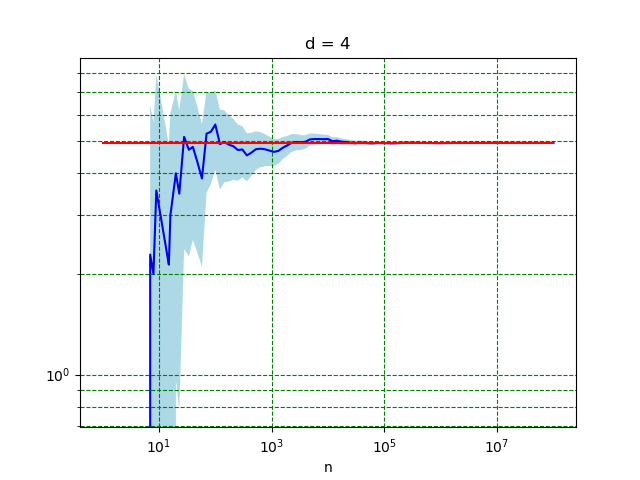
\includegraphics[width=8cm]{../python/report1_monte_carlo/out/r2plot4d.png}
\end{center}
\caption{4次元球の体積が理論値へと収束していく様子}
\end{figure}

\begin{figure}[H]
\begin{center}
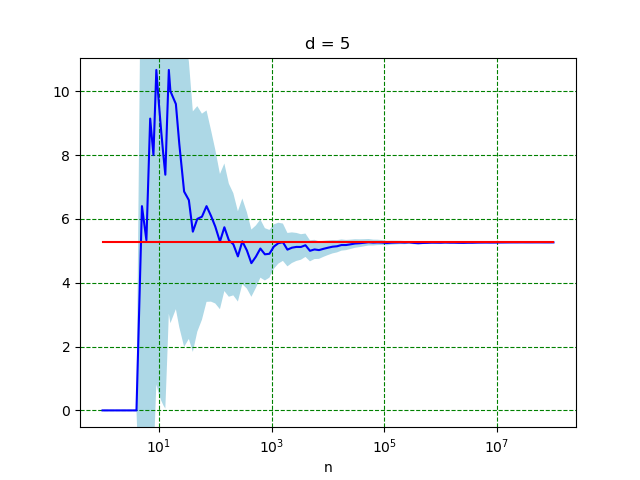
\includegraphics[width=8cm]{../python/report1_monte_carlo/out/r2plot5d.png}
\end{center}
\caption{5次元球の体積が理論値へと収束していく様子}
\end{figure}

\begin{figure}[H]
\begin{center}
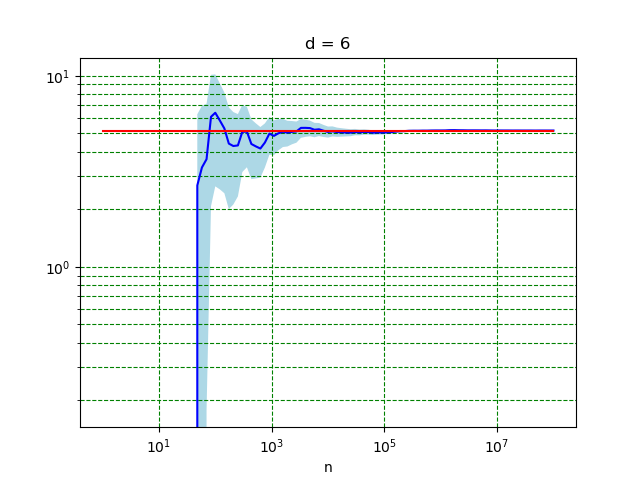
\includegraphics[width=8cm]{../python/report1_monte_carlo/out/r2plot6d.png}
\end{center}
\caption{6次元球の体積が理論値へと収束していく様子}
\end{figure}

\begin{figure}[H]
\begin{center}
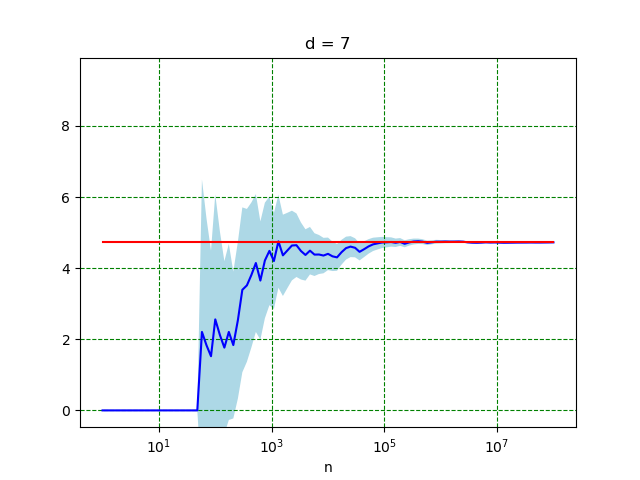
\includegraphics[width=8cm]{../python/report1_monte_carlo/out/r2plot7d.png}
\end{center}
\caption{7次元球の体積が理論値へと収束していく様子}
\end{figure}

\begin{figure}[H]
\begin{center}
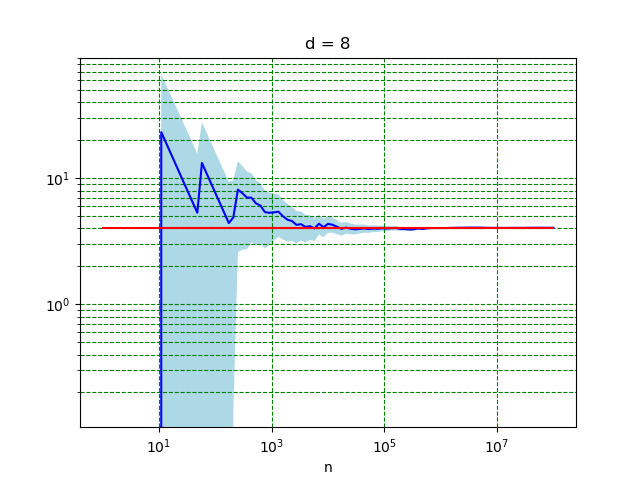
\includegraphics[width=8cm]{../python/report1_monte_carlo/out/r2plot8d.png}
\end{center}
\caption{8次元球の体積が理論値へと収束していく様子}
\end{figure}

\begin{figure}[H]
\begin{center}
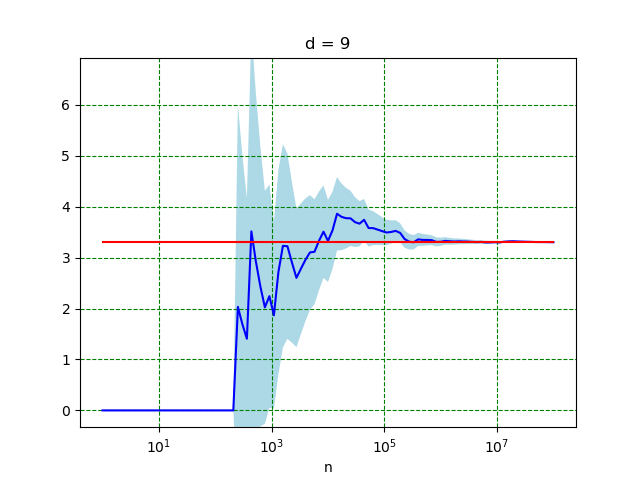
\includegraphics[width=8cm]{../python/report1_monte_carlo/out/r2plot9d.png}
\end{center}
\caption{9次元球の体積が理論値へと収束していく様子}
\end{figure}

\begin{figure}[H]
\begin{center}
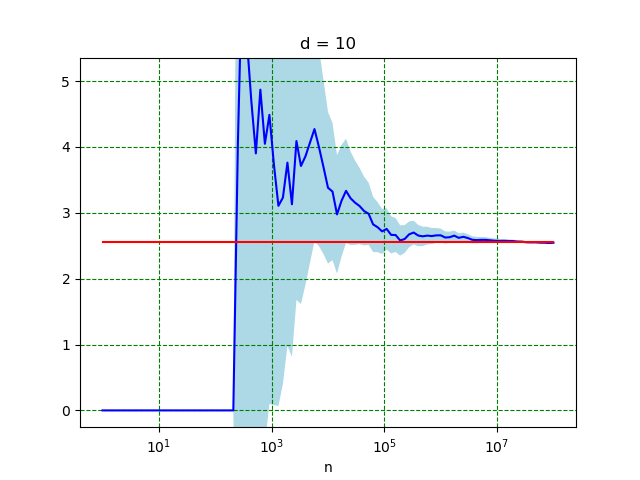
\includegraphics[width=8cm]{../python/report1_monte_carlo/out/r2plot10d.png}
\end{center}
\caption{10次元球の体積が理論値へと収束していく様子}
\end{figure}

\begin{figure}[H]
\begin{center}
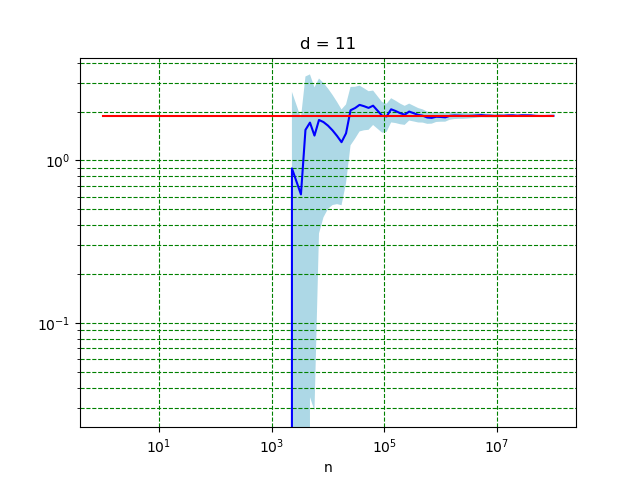
\includegraphics[width=8cm]{../python/report1_monte_carlo/out/r2plot11d.png}
\end{center}
\caption{11次元球の体積が理論値へと収束していく様子}
\end{figure}

\begin{figure}[H]
\begin{center}
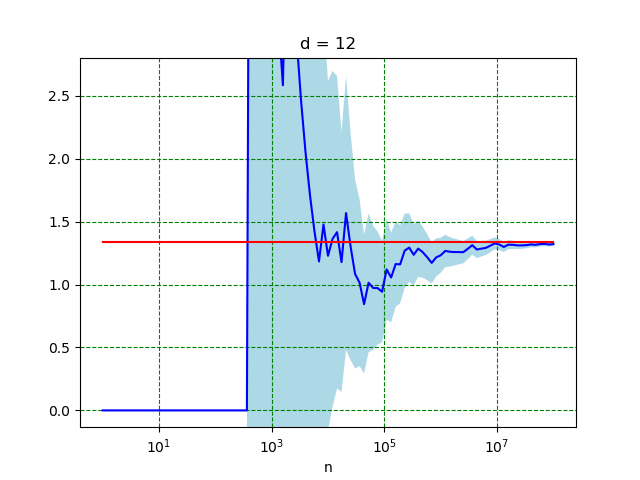
\includegraphics[width=8cm]{../python/report1_monte_carlo/out/r2plot12d.png}
\end{center}
\caption{12次元球の体積が理論値へと収束していく様子}
\end{figure}

\begin{figure}[H]
\begin{center}
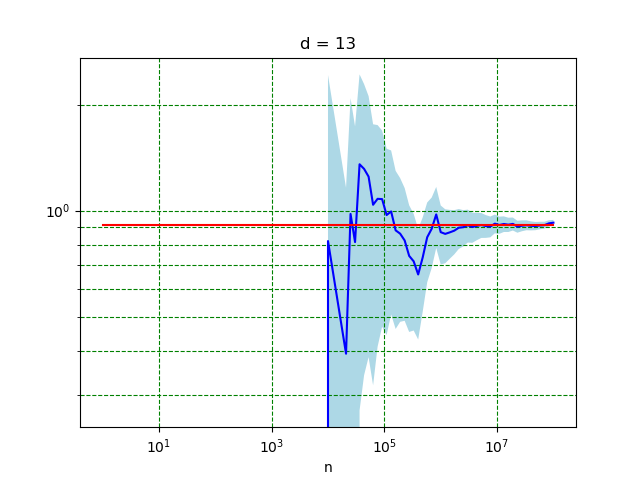
\includegraphics[width=8cm]{../python/report1_monte_carlo/out/r2plot13d.png}
\end{center}
\caption{13次元球の体積が理論値へと収束していく様子}
\end{figure}

\begin{figure}[H]
\begin{center}
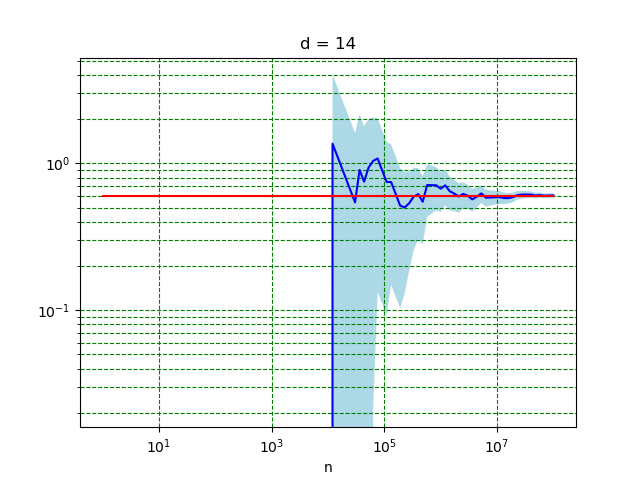
\includegraphics[width=8cm]{../python/report1_monte_carlo/out/r2plot14d.png}
\end{center}
\caption{14次元球の体積が理論値へと収束していく様子}
\end{figure}

\begin{figure}[H]
\begin{center}
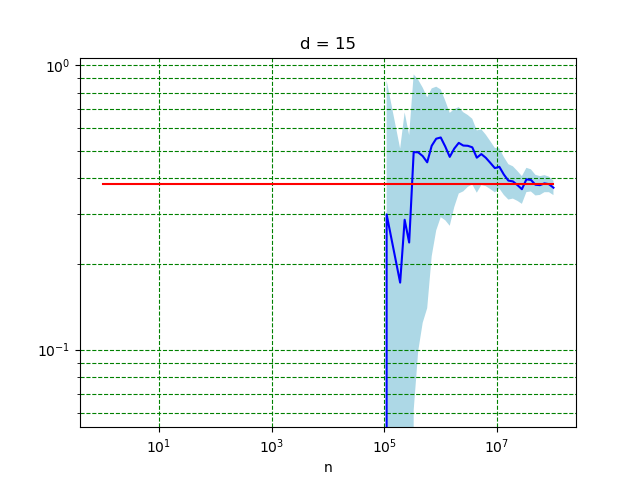
\includegraphics[width=8cm]{../python/report1_monte_carlo/out/r2plot15d.png}
\end{center}
\caption{15次元球の体積が理論値へと収束していく様子}
\end{figure}

\begin{figure}[H]
\begin{center}
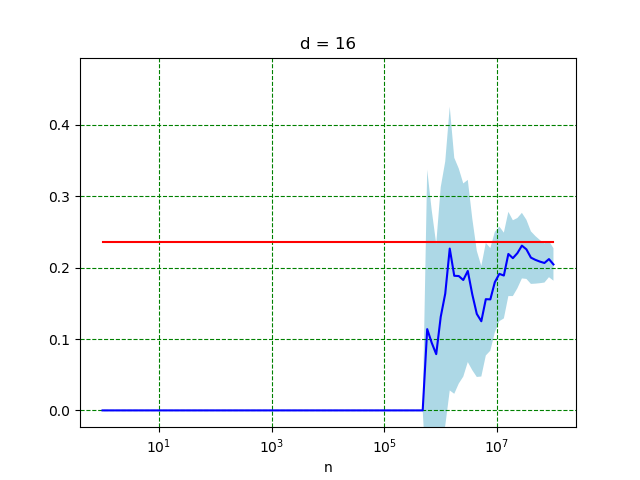
\includegraphics[width=8cm]{../python/report1_monte_carlo/out/r2plot16d.png}
\end{center}
\caption{16次元球の体積が理論値へと収束していく様子}
\end{figure}

\begin{figure}[H]
\begin{center}
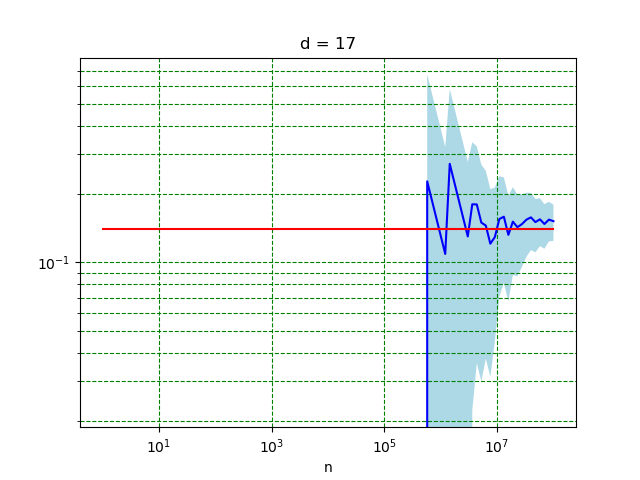
\includegraphics[width=8cm]{../python/report1_monte_carlo/out/r2plot17d.png}
\end{center}
\caption{17次元球の体積が理論値へと収束していく様子}
\end{figure}

\begin{figure}[H]
\begin{center}
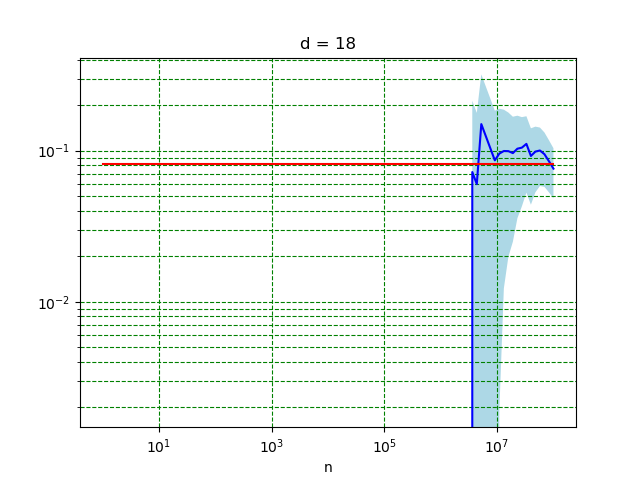
\includegraphics[width=8cm]{../python/report1_monte_carlo/out/r2plot18d.png}
\end{center}
\caption{18次元球の体積が理論値へと収束していく様子}
\end{figure}

\begin{figure}[H]
\begin{center}
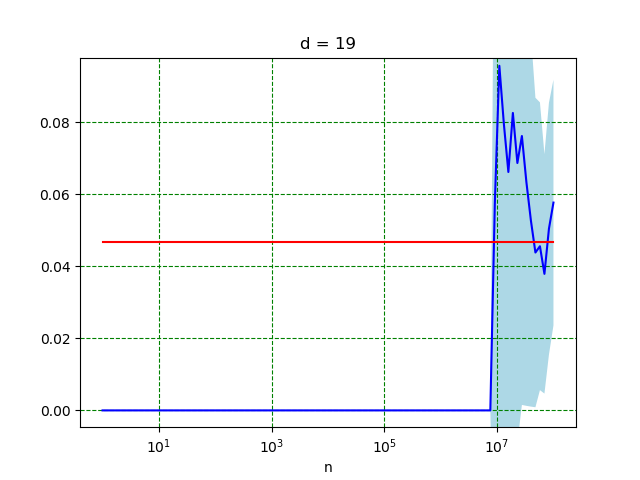
\includegraphics[width=8cm]{../python/report1_monte_carlo/out/r2plot19d.png}
\end{center}
\caption{19次元球の体積が理論値へと収束していく様子}
\end{figure}

\begin{figure}[H]
\begin{center}
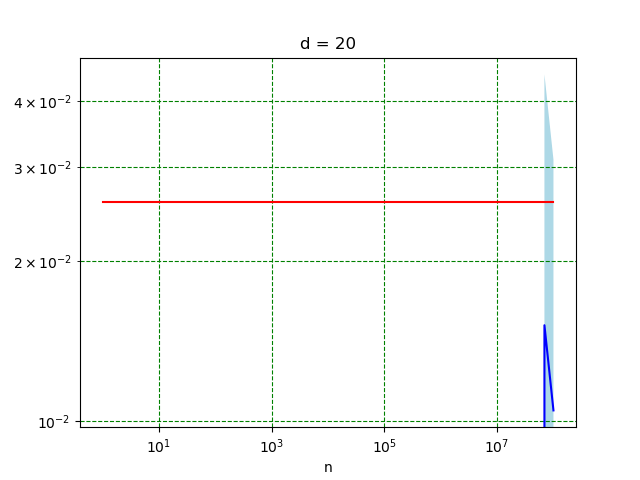
\includegraphics[width=8cm]{../python/report1_monte_carlo/out/r2plot20d.png}
\end{center}
\caption{20次元球の体積が理論値へと収束していく様子}
\end{figure}

\subsection{考察}
誤差は試行回数が大きくなるにつれて小さくなるのが視覚的にわかったが、次元$d$が大きくなるにつれて、収束が遅くなり、同じだけ誤差が小さくなるのによりたくさんの点が必要なことがうかがえる。

また、誤差は点が一つ以上球の中に入ってからは、概ね理論値を含むような範囲をとっていることがわかる。

誤差は点が一つ以上球の中に入ってからはいない状態では誤差は0になってしまっている。本来はこの状態でも理論値を含むような値\footnote{例えば無限}をとるべきであるがこうなってしまうのは、試行回数が十分大きいと仮定した上で得られた標本分散をそのまま母分散としてしまっている点にあると思われる。本来は試行回数が小さい場合も考慮して、標本分散から母分散を推定すべきであるが、今回の課題の趣旨とずれるためこれについての作業は行わなかった。機会があったら行いたい。

\section{次元を変えたときの超球の体積の変化}
\subsection{内容}
また、次元を変えたときの超球の体積の変化を横軸次元、縦軸体積と誤差$1.96 \sigma$としてプロットした。試行回数は$10^8$回行った。

\subsection{ソースコード}
C++ のコードは\ref{s-variance}と同一である。

plotmulti\_v\_s.py
\begin{lstlisting}
# -*- coding: utf-8 -*-

import matplotlib.pyplot as plt
import numpy as np
import csv

from matplotlib import ticker


def main():
  data = []
  with open('../../cpp/out/v_s_plot.csv') as f:
      rows = csv.reader(f, quoting=csv.QUOTE_NONNUMERIC)
      for row in rows:
          data.append(row)

  # print(data)
  d = [row[0] for row in data]
  v = [row[1] for row in data]
  error = [row[2] for row in data]

  # v_plus_error = [e + error[i] for i, e in enumerate(v)]
  # v_minus_error = [e - error[i] for i, e in enumerate(v)]

  # plt.plot('o')
  # plt.axes(yerr=error).errorbar()
  # plt.plot(n, v_plus_error, 'b', linestyle='solid')
  # plt.plot(n, v_minus_error, 'b', linestyle='solid')
  plt.errorbar(d, v, yerr=error, fmt='--o', ecolor='g')


  # plt.axes().set_ylim(ymin=-max(v)*0.1, ymax=max(v_plus_error)*1.1)
  # plt.axes().set_ylim(ymin=-0.1*v_theory[0], ymax=2.1*v_theory[0])
  plt.axes().set_xticks(np.arange(2, 21, step=1))
  # plt.xscale('log')
  # plt.yscale('log')
  plt.grid(True, which="both", axis='both', ls="--", color="grey")
  plt.xlabel('d')
  plt.ylabel('v ± 1.96 σ')
  plt.title('n = 10 ** 8')
  plt.savefig('out/v_s_plot.eps')
  plt.savefig('out/v_s_plot.png')
  plt.show()


if __name__ == "__main__":
  main()
\end{lstlisting}

\subsection{結果}

\begin{figure}[H]
\begin{center}
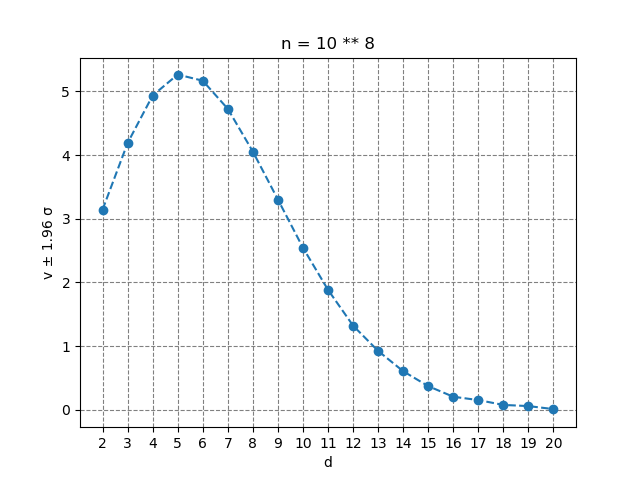
\includegraphics[width=8cm]{../python/report1_monte_carlo/out/v_s_plot.png}
\end{center}
\caption{各次元ごとにおける超球の体積$V_n(R)$とその誤差 $1.96 \sigma$(誤差が小さすぎて見えないが…)}
\end{figure}

\subsection{考察}
誤差$1.96 \sigma$も縦軸にプロットしているのだが
体積は5次元のときに最も大きいことがわかる。$10^8$回の試行で低次元においてモンテカルロ法で求めた超球の体積が理論値に収束していることは\ref{s-variance}で確かめたし、この図から誤差はかなり小さいことがうかがえるので\footnote{というより誤差が小さすぎてそもそもプロットされているかもわからない。}、このプロットが正確であることはいうまでもないだろう。

\begin{thebibliography}{99}
\bibitem{wiki-monte-carlo}
https://ja.wikipedia.org/wiki/モンテカルロ法

\bibitem{wiki-volume-n-ball}
https://ja.wikipedia.org/wiki/超球の体積

\end{thebibliography}

\end{document}
